\documentclass[hidelinks,12pt,a4paper]{article}
\usepackage[utf8]{inputenc}
\usepackage{tikz}
\usetikzlibrary{decorations.pathreplacing}
\usepackage{microtype}
\usepackage{amsmath}
\usepackage{amsfonts}
\usepackage{amssymb}
\usepackage{xargs}
\usepackage[parfill]{parskip}
\usepackage[margin=1.3in]{geometry}
\usepackage{tabularx}
\usepackage{float}
\usepackage{amsthm}
\usepackage{hyperref}
\usepackage{subcaption}
\usepackage{lscape}
\usepackage{caption}

%\usepackage{ccfonts}
%\usepackage[adobe-utopia]{mathdesign}
%\usepackage{eucal}
%\usepackage{arev}
%\usepackage[T1]{fontenc}
%\usepackage{fontspec}
%\setmainfont{Asana-Math}
%\usepackage[adobe-utopia]{mathdesign}
\usepackage{libertinus}
\usepackage{fdsymbol}
\usepackage[T1]{fontenc}

\usepackage[ruled,vlined,linesnumbered,noend]{algorithm2e}
\usepackage{setspace}

%\def\arraystretch{1.2}

\newcommand{\Qc}{\mathcal{Q}}
\newcommand{\Sc}{\mathcal{S}}
\newcommand{\E}{\mathbb{E}}
\newcommand{\Act}{\mathrm{Act}}
\newcommand{\Ac}{\mathcal{A}}
\newcommand{\dt}{\matrm{\ d}}
\newcommand{\KL}{\mathrm{KL}}
\newcommand{\Af}{\mathbf{A}}
\newcommand{\bfat}{\mathbf{b}}
\newcommand{\xf}{\mathbf{x}}
\newcommand{\af}{\mathbf{a}}
\newcommand{\yf}{\mathbf{y}}
\newcommand{\Df}{\mathbf{D}}
\newcommand{\cf}{\mathbf{c}}
\newcommand{\ef}{\mathbf{e}}
\newcommand{\gf}{\mathbf{g}}
\newcommand{\df}{\mathbf{d}}
\newcommand{\Lc}{\mathcal{L}}
\newcommand{\Uc}{\mathcal{U}}
\newcommand{\Be}{\mathrm{Be}}
\newcommand{\Mult}{\mathrm{Mult}}
\newcommand{\Nc}{\mathcal{N}}
\newcommand{\Fc}{\mathcal{F}}
\newcommand{\R}{\mathbb{R}}
\newcommand{\N}{\mathbb{N}}
\newcommand{\Cov}{\mathrm{Cov}}
\newcommand{\Var}{\mathrm{Var}}
\newcommand{\dom}{\mathrm{dom}}
\newcommand{\st}{\text{subject to}}

\DeclareMathOperator*{\argmax}{\arg\max}
\DeclareMathOperator*{\argmin}{\arg\min}
\newcommand{\pdata}{p_\mathrm{data}}
\newcommand{\pmodel}{p_\mathrm{model}}
\numberwithin{equation}{section}


\newcommand{\idx}{\varphi}
\newcommand{\varidx}{\psi}
\newcommand{\move}[3]{#1_{#2\rightarrow #3}}
\newcommand{\image}{\mathrm{image}}
\newcommand{\minimize}{\text{minimize}}
\renewcommand{\iff}{\quad\text{iff}\quad}

% \newtheoremrep{theorem}{Theorem}[section]
% \newtheoremrep{corollary}{Corollary}[theorem]
% \newtheoremrep{lemma}[theorem]{Lemma}
\newtheorem{definition}{Definition}[section]

\usepackage[appendix=append]{apxproof}
\newtheoremrep{theorem}{Theorem}[section]
\newtheoremrep{corollary}{Corollary}[theorem]
\newtheoremrep{lemma}[theorem]{Lemma}

\makeatletter
\newcommand*{\algotitle}[2]{%
  \stepcounter{algocf}%
  \hypertarget{algocf.title.\theHalgocf}{}%
  \NR@gettitle{#1}%
  \label{#2}%
  \addtocounter{algocf}{-1}%
}
\makeatother

\title{A Local Search Algorithm for Cubic Clustering}
\author{Hans Harder, TU Dresden}
\date{}

\begin{document}

\maketitle

\tableofcontents
\newpage


\section{Notation}
Let $A$ be some set. We will denote the set $\{ \{ a_1, \dots, a_k \} \subseteq A : a_1,\dots,a_k\ \text{distinct}\},$ which contains all $k$-ary subsets of $A$, by $\binom{A}{k}$. For the same set $A$, $P_A$ denotes the set of all partitions of $A$. For a partition $\Pi \in P_A$ and an element $a \in A$, $[a]_\Pi$ denotes the set in $\Pi$ that contains $a$, of which there is exactly one. If $A$ is finite, $\Uc(A)$ denotes the uniform distribution over $A$, i.e. the distribution that assigns every element in $A$ the same probability (namely: $1/|A|$). If we want to indicate that a random variable ${\bf X}$ has probability distribution $\mathcal{Q}$, we will write ${\bf X} \sim \mathcal{Q}$. If $f$ is a function from the domain of a random variable ${\bf X} \sim \mathcal{Q}$ to the real numbers, its expected value is written as $\E_{{\bf X} \sim \mathcal{Q}}\left[f({\bf X})\right]$ and defined as $\E_{{\bf X} \sim \mathcal{Q}} \left[f({\bf X})\right] = \sum_{i=1}^n \mathcal{Q}(x_i) f(x_i)$, if the domain of ${\bf X}$ is finite and given by $\{x_1,\dots,x_n\}$ (we will only consider finite domains).


\section{Introduction}
This work is concerned with the partioning problem with respect to a given finite set $V$, with a cost structure defined over 3-ary subsets of $V$. The considered problem is hard in many respects: one, the amount of possible partitions grows large very fast (with growing $|V|$). Two, even computing the objective function for a given partition is prohibitive, since summing over all $3$-ary subsets takes almost $|V|^3$ steps (and to add to that, not even $|V|^2$ steps are feasible if $|V|$ becomes larger). Thus, we are interested in a way of approximately solving this problem by the use of local search algorithms and some considerations on the objective function. Since the No-Free-Lunch-Theorem (Wolpert et al., \cite{wolpert1995no}) implies that there is no such thing as the ``best'' local search algorithm for arbitrary cost-structures, we want to omit too much focus on specific search algorithms and rather focus on some shared difficulties, e.g. the efficient... 
\begin{itemize}
    \item ...representation of partitions,
    \item ...enumeration of ``neighbours'' for a given partition (possibly in random order)
    \item ...computation (or estimation) of the given cost function and cost-improvements.
\end{itemize}
The problem is given as follows. Let $V = \{ v_1,\dots,v_n \}$ be a finite set, which we will call the set of vertices. Associated with this set are functions $$ c,c': \tbinom{V}{3} \mapsto \R $$ which define a cost-structure on $3$-ary subsets of $V$. For a subset $\{u,v,w\} \in \binom{V}{3}$ and a given partition $\Pi \in P_V$, we define the cost of $\{u,v,w\}$ with respect to $\Pi$ as  
\begin{align*}
    \ell(\{u,v,w\},\Pi) = \begin{cases}
        c(\{u,v,w\}) & \text{if}\ [u]_\Pi \neq [v]_\Pi, [u]_\Pi \neq [w]_\Pi, [w]_\Pi \neq [v]_\Pi \\
        c'(\{u,v,w\}) & \text{if}\ [u]_\Pi = [v]_\Pi = [w]_\Pi \\
        0 & \text{otherwise.}
    \end{cases}
\end{align*}
This can be interpreted as follows: whenever $u,v$ and $w$ are part of pairwise different sets in $\Pi$, the cost of $\{u,v,w\}$ is equal to the costs as defined by $c$. If they are part of the same set, the cost of $\{u,v,w\}$ is equal to the costs as defined by $c'$. Otherwise, if neither of the above is the case, the cost of $\{u,v,w\}$ is just $0$. Based on this definition, we are confronted with problems of the form
\begin{align*}
    \Pi^* = \argmin_{\Pi \in P_V} \sum\nolimits_{\{u,v,w\} \in \binom{V}{3}} \ell(\{u,v,w\},\Pi),
\end{align*}
i.e. we wish to find a partition $\Pi^*$ of $V$ that minimizes some objective function over $3$-ary subsets of $V$. 
\\
In the following section \emph{\nameref{sec:indexings}}, we will discuss an efficient way of representing partitions, e.g. with respect to their space requirements. Afterwards, in section \emph{\nameref{sec:move-operation}}, we consider ways of transforming these representation such that we are able to efficiently generate a neighbourhood (in random order) for each partition. In section \emph{\nameref{sec:objective-function}} we will investigate how the change in the objective function can be computed or estimated, with respect to the neighbourhood of a given partition. The penultimate part \emph{\nameref{sec:algorithms}} contains a theoretic discussion on how the proposed settings influence the runtime of a simple greedy search algorithm, which will be evaluated in section \emph{\nameref{sec:experiments}}. Proofs for Lemmas and Theorems that are shown in this work can be found in the appendix.
\section{Indexings as Proxies for Partitions}\label{sec:indexings}
Since we want to use a local search algorithm that iteratively finds better solutions (partitions in this case), we want to consider on how we want to represent said partitions. One may represent a partition as a set of sets of vertices, which is probably the most straight-forward approach. On the one hand, the required space is linear in $|V|$. But on the other hand, this comes with a few problems: checking if two vertices are part of the same set, and the removal and the addition of a vertex from or to a set all require $|V|$ steps in the worst case (if all vertices have the same set). A last problem is that one has to gurantee feasibility at every step, i.e. that every solution is indeed a partition. A second idea might be to store a partition as a $|V| \times |V|$ boolean matrix, where every row corresponds to a vertex and every column to a set in the partition, and an entry at position $i,j$ would mean ``vertex $i$ is part of set $j$'' if $1$ and ``vertex $i$ is not part of set $j$'' if $0$. This would alleviate some of the above problems, since looking up, removal or addition of vertices to sets would take constant time in the worst case. However, storing a partition would require $|V|^2$ units of space, which might become problematic when $|V|$ is large or when considering multiple partitions at once.

Therefore, we will use the following concept of indexings (which induce equivalence relations on $V$) to solve the above problems, i.e. to simplify and speed up operations on partitions. Every vertex is mapped to a number (index) which indicates the set in the partition we want this vertex to be a part of. If multiple vertices are mapped to the same index, they will be part of the same set in the partition. Since there are at maximum $|V|$ sets in a partition of $V$ (every vertex is assigned its own set, i.e. the indexing is bijective), we restrict to indices between $1$ and $|V|$. Note that every indexing can be stored in space $O(|V|)$.


\begin{figure}[ht]
    \centering
    \begin{tikzpicture}
    
    \foreach \s in {1,...,5} {
        \node[draw, circle] (vl\s) at (0,5-\s) {$v_\s$};
        \node[draw, circle] (nl\s) at (2,5-\s) {$\s$};
        \node[draw, circle] (nr\s) at (4,5-\s) {$\s$};
        \node[draw, circle] (vr\s) at (6,5-\s) {$v_\s$};
    }

    \draw[->] (vl1) -- (nl2);
    \draw[->] (vl2) -- (nl2);
    \draw[->] (vl3) -- (nl5);
    \draw[->] (vl4) -- (nl5);
    \draw[->] (vl5) -- (nl5);

    \draw[->] (vr1) -- (nr1);
    \draw[->] (vr2) -- (nr1);
    \draw[->] (vr3) -- (nr3);
    \draw[->] (vr4) -- (nr3);
    \draw[->] (vr5) -- (nr3);

    \draw[->] (nl2) -- (nr1);
    \draw[->] (nl5) -- (nr3);


    \draw [decorate,decoration={brace,amplitude=5pt,mirror,raise=4ex}](0.1,0) -- (1.9,0) node[midway,yshift=-3em]{$\idx$};

    \draw [decorate,decoration={brace,amplitude=5pt,mirror,raise=4ex}](2.1,0) -- (3.9,0) node[midway,yshift=-3em]{$\lambda$};

    \draw [decorate,decoration={brace,amplitude=5pt,mirror,raise=4ex}](4.1,0) -- (5.9,0) node[midway,yshift=-3em]{$\varidx$};

    \node at (0,5) {$\Pi(\idx)$};
    \draw [decorate,decoration={brace,amplitude=5pt,raise=4ex},xshift=-4pt,yshift=0pt,align=right](0,-0.4) -- (0,2.4) node [black,midway,xshift=-2.8cm] {$[v_3]_\idx = [v_4]_\idx = [v_5]_\idx$ \\ $= \{v_3,v_4,v_5\}$};
    \draw [decorate,decoration={brace,amplitude=5pt,raise=4ex},xshift=-4pt,yshift=0pt,align=right](0,2.6) -- (0,4.4) node [black,midway,xshift=-2.1cm] {$[v_1]_\idx = [v_2]_\idx$\\ $= \{v_1,v_2\}$};
    \draw[rounded corners=5pt, dashed] (-0.5,-0.45) rectangle (0.5,2.45);
    \draw[rounded corners=5pt, dashed] (-0.5,3-0.45) rectangle (0.5,3+1.45);

    \node at (6,5) {$\Pi(\varidx)$};
    \draw[rounded corners=5pt, dashed] (6-0.5,-0.45) rectangle (6+0.5,2.45);
    \draw[rounded corners=5pt, dashed] (6-0.5,3-0.45) rectangle (6+0.5,3+1.45);

    \end{tikzpicture}
    \captionsetup{width=.9\linewidth}
    \caption{Illustration of two indexings $\idx,\varidx$ with corresponding partitions and proof of equality through part (b) of Theorem \ref{theorem:equal_indexings}.}\label{fig:indexings}
\end{figure}

\begin{definition}
    Let $V = \{ v_1,v_2,\dots, v_n \}$ be a set of vertices. An indexing of $V$ is a mapping $\idx \in \{ 1,\dots,n \}^V = [n]^V$ that associates every vertex with a number from 1 to $n$. \label{def:indexings}
\end{definition}

\begin{definition}
    Let $\idx$ be an indexing of $V$. The partition induced by $\idx$ is defined as
    \begin{equation}
        \Pi(\idx)= \{ [v]_\idx : v \in V \}, \label{eq:indexing}
    \end{equation}
    where $[v]_\idx = \{ w \in V : \idx(w) = \idx(v) \}$. \label{def:indexing_partition}
\end{definition}

Based on definition \ref{def:indexings} and \ref{def:indexing_partition}, we are able to obtain some immediate results. First, we are able to use indexings as representations for partitions, i.e. for every partition, there is some indexing that yields that very partition (Lemma \ref{lemma:indexing_partition}). And two, we obtain a criterion that makes it possible to check when two vertices share the same set in the partition (Lemma \ref{lemma:indexing_same_set}).  

\begin{samepage}
    \begin{lemmarep}
        $\Pi$ partitions $V$ if and only if there exists an indexing of $V$ that induces $\Pi$.\label{lemma:indexing_partition}
    \end{lemmarep}
\end{samepage}
\begin{proof}
    First, we will show the direction from left to right. Let $\Pi = \{U_1,\dots,U_m\}$, $1\leq m \leq n$, be a partition of $V$. For all vertices $v$ with corresponding set $U_i$ in $\Pi$ (of which there is exactly one), we define $\idx(v) = i$. For a $j \in \{1,\dots,m\}$ we then obtain $\idx^{-1}(j) = U_j$. But then $\Pi(\idx) = \Pi$, i.e. $\Pi$ is induced by $\idx$. 
    \\
    The other direction requires us to prove that every indexing induces a partition of $V$. I.e., for an indexing $\idx$ of $V$ with $\Pi(\idx)=\Pi$, we need to check the following requirements:
    \begin{enumerate}
        \item $\emptyset \not\in \Pi$:\quad This is obvious from \eqref{eq:indexing}, since every element $[v]_\idx \in \Pi$ contains $v$. %https://en.wikipedia.org/wiki/Partition_of_a_set
        \item $\bigcup_{U \in \Pi} U = V$:\quad ``$\subseteq$'' is obvious. For ``$\supseteq$'', take a vertex $v$. Then, $v \in [v]_\idx$ and since $[v]_\idx \in \Pi(\idx)$, we obtain $v \in \bigcup_{U \in \Pi} U$.
        \item if $U_1,U_2 \in \Pi$ and $U_1 \neq U_2$, then $U_1 \cap U_2 = \emptyset$:\quad Take two $U_1, U_2 \in \Pi$ with $U_1 \neq U_2$ such that $U_1 = [w]_\idx$ and $U_2 = [u]_\idx$ for two vertices $w$ and $u$. Assume for a contradiction that $U_1 \cap U_2 \neq \emptyset$, i.e. there exists $v \in U_1 \cap U_2$. But then $v \in [w]_\idx$ and $v \in [u]_\idx$. Thus, $\idx(v) = \idx(w) = \idx(u)$, which cannot be the case, since that would imply $U_1 = U_2$.
    \end{enumerate}
    This completes the proof.
\end{proof}

\begin{samepage}
    \begin{lemmarep}
        Let $\idx$ be an indexing of $V$. For all vertices $v,u$, we have $\idx(v) = \idx(u)$ if and only if $v$ and $u$ are part of the same set in $\Pi(\idx)$. \label{lemma:indexing_same_set}
    \end{lemmarep}
\end{samepage}
\begin{proof}
    For the direction from left to right, take $v,u\in V$ such that $\idx(v)=\idx(u)$. Then $v,u \in [v]_\idx = [u]_\idx \in \Pi(\idx)$, i.e. they are part of the same set. For the other direction, we will show the contraposition. Take $v,u\in V$ such that $\idx(v)\neq \idx(u)$. Clearly, $v \in [v]_\idx$ and $v \not\in [u]_\idx$ as well as $u \in [u]_\idx$ and $u \not\in [v]_\idx$. Therefore $[v]_\idx \neq [u]_\idx$. Since by Lemma \ref{lemma:indexing_partition}, $\Pi(\idx)$ is a partition and $[v]_\idx$ and $[u]_\idx$ are distinct sets in $\Pi(\idx)$, $[v]_\idx$ is the only set that contains $v$ and vice versa for $[u]_\idx$ and $u$. Thus, $v$ and $u$ cannot be part of the same set in $\Pi(\idx)$. 
\end{proof}

Since we want to use indexings in order to define transformations on partitions, we are interested in the question when two indexings are ``equal'', in the sense that they induce the same partition. This is characterized in part by Theorem \ref{theorem:equal_indexings}.

\begin{samepage}
    \begin{theoremrep}
        If $\idx,\varidx$ are two indexings of $V$, then the following statements are equivalent:
        \begin{enumerate}
            \item[(a)] $\Pi(\idx)=\Pi(\varidx)$
            \item[(b)] there is a bijection $\lambda : \image(\idx) \rightarrow \image(\varidx)$\footnote{$\image(\idx)$ means the image of $\idx$, i.e. $\image(\idx)=\{ \idx(v) \}_{v \in V}$.} such that $\lambda(\idx(v)) = \varidx(v)$ \\ for all $v \in V$
            \item[(c)] for all vertices $v,w$, $\idx(w) = \idx(v)$ if and only if $\varidx(w) = \varidx(v)$
        \end{enumerate} \label{theorem:equal_indexings}
    \end{theoremrep}
\end{samepage}
\begin{proof}
    We will start with the direction from (a) to (b). Let $\idx$, $\varidx$ be two indexings of $V$ with $\Pi(\idx) = \Pi(\varidx)$. We define $\lambda : \image(\idx)\rightarrow \image(\varidx)$ as follows. For all $k \in \image(\idx)$, associate a vertex $v$ such that $\idx(v)=k$. Then define $\lambda(k)=\varidx(v)$. It remains to show that $\lambda$ fulfills the requirements in (b):
    \begin{enumerate}
        \item $\lambda$ is bijective:\quad Since every element in $\image(\idx)$ corresponds to a set in $\Pi(\idx)$, and vice versa for $\image(\varidx)$ and $\Pi(\varidx)$, we get $|\image(\idx)|=|\Pi(\idx)|=|\Pi(\varidx)|=|\image(\varidx)|$. Since $\image(\idx)$ and $\image(\varidx)$ are also finite, it suffices to show injectivity of $\lambda$ in order to prove bijectivity. Assume for a contradiction that $\lambda$ is not injective, i.e. there are $v_1,v_2 \in V, \idx(v_1) \neq \idx(v_2)$, such that $\lambda(\idx(v_1))=\lambda(\idx(v_2))=\varidx(v_1)=\varidx(v_2)$. Thus, by application of Lemma \ref{lemma:indexing_same_set}, there must be a set in $\Pi(\varidx)$ that contains $v_1$ and $v_2$, while there is no set in $\Pi(\idx)$ that has both vertices in it. But then $\Pi(\idx)\neq \Pi(\varidx)$. Contradiction.
        \item For all vertices $v$, $\lambda(\idx(v)) = \varidx(v)$: \quad Take an arbitrary vertex $v$ and let $\idx(v) = k \in \image(\idx)$. Let $\bar{v}$ be the vertex that was previously associated with $k$ in the definition of $\lambda$, i.e. the vertex for which $\idx(\bar{v})=k = \idx(v)$ and $\lambda(\idx(\bar{v}))=\varidx(\bar{v})$ holds. Assume for a contradiction that $\varidx(v)\neq \varidx(\bar{v})$. By Lemma \ref{lemma:indexing_same_set}, this yields that there is no set in $\Pi(\varidx)$ that contains both $v$ and $\bar{v}$, while there is one in $\Pi(\idx)$. But then again $\Pi(\idx) \neq \Pi(\varidx)$, i.e. a contradiction. Thus, $\lambda(\idx(v)) = \lambda(\idx(\bar{v})) = \varidx(\bar{v}) = \varidx(v)$. 
    \end{enumerate}
    This concludes this direction. For the direction from (b) to (c), let $\lambda$ be a bijection between the images of two indexings $\idx, \varidx$ of $V$ that fulfills the requirements in (b). Let $w,v$ be two arbitrary vertices; then
    \begin{align*}
        \idx(w) = \idx(v) &\quad\text{iff}\quad \lambda(\idx(w)) = \lambda(\idx(v)) &(*) \\ 
        &\quad\text{iff}\quad \varidx(w) = \varidx(v) &(**)
    \end{align*}
    The first identity $(*)$ works since $\lambda$ is a bijection and the second $(**)$ since $\lambda(\idx(w))=\varidx(w)$ for all vertices $w$.
    The remainder (c) to (a) is relatively trivial: If we assume premise (c), then
    \begin{align*}
        U \in \Pi(\idx) &\quad\text{iff}\quad U = [v]_\idx \text{ for a vertex $v$} \\
        &\quad\text{iff}\quad U = \{ w \in V : \idx(w) = \idx(v) \} \text{ for a vertex $v$} \\
        &\quad\text{iff}\quad U = \{ w \in V : \varidx(w) = \varidx(v) \} \text{ for a vertex $v$} \\ 
        &\quad\text{iff}\quad U = [v]_{\varidx} \text{ for a vertex $v$} \\
        &\quad\text{iff}\quad U \in \Pi(\varidx),
    \end{align*}
    which shows $\Pi(\idx)=\Pi(\varidx)$.
\end{proof}

If the task is to determine whether two induced partitions $\Pi(\idx)$, $\Pi(\varidx)$ for given indexings $\idx,\varidx$ of $V$ are equal, the result of Theorem \ref{theorem:equal_indexings} might be useful: instead of explicitly computing the resulting partitions and checking if both sets are equal, one can simply determine whether a fitting bijection $\lambda$ exists, which is arguably easier. In fact, one can construct $\lambda$ as in the first part of the proof of Theorem \ref{theorem:equal_indexings} and then check whether the result is a bijection or not. Figure \ref{fig:indexings} illustrates two indexings, their partitions and some of the findings of Theorem \ref{theorem:equal_indexings}.
\section{Move-Operation on Indexings}\label{sec:move-operation}

We will now define the ``move''-operation on indexings, which transforms an indexing into another indexing by changing the assigned index of a vertex. The effect this has on the induced partition is that the respective vertex is ``taken'' from its original set\footnote{i.e. the set $[v]_\idx$} and then ``put into'' some other set. This is then defined as
\begin{equation} 
\move{\idx}{ v}{ k}(u) = \begin{cases}
    \idx(u) & u \neq v, \\ 
    k & u = v
\end{cases} \label{eq:move-operation}
\end{equation} 
for every vertex $u$. The operation takes as input an indexing $\idx$, a vertex $v$ and new index $k$ and outputs a new indexing that is essentially the same as $\idx$, with the only difference being that $v$ is mapped to $k$ instead of whatever it was mapped to before.

\subsection{Move-Enumeration}

In many cases, there are multiple ways of moving one vertex to different indices while still inducing the same partition afterwards. For example, if $v$ is an arbitrary vertex, $\idx$ is an indexing of $V$ with pairwise different $k_1,k_2$ such that there is no vertex $u$ with $\idx(u) = k_1$ or $\idx(u) = k_2$, then moving $v$ to $k_1$ or $k_2$ yields that while $\move{\idx}{v}{k_1}$ and $\move{\idx}{v}{k_2}$ are different indexings, their induced partitions are the same: $\Pi(\move{\idx}{v}{k_1}) = \Pi(\move{\idx}{v}{k_2})$. Based on this observation we are interested in an efficient way of enumerating all possible ``moves'' of a vertex with respect to the induced partitions without enumerating too much or having to double-check whether two move-operations induce the same partition. Hence, consider algorithm \emph{\nameref{alg:moveenum}}, which aims at finding a solution to this problem.

\begin{algorithm}[ht]
    \algotitle{ME}{alg:moveenum.title}
    \SetAlgoLined
    \DontPrintSemicolon
    \KwIn{Set of vertices $V$ with indexing $\idx$}
    \KwResult{Sequence of moves $(w_1,k_1),\dots,(w_m,k_m)$ }
    Let $<$ be some linear order on $V$ \label{alg:moveenum:l1} \;
    Let $\mathcal{N} := \{1,\dots,n\}\backslash \image(\idx)$  \label{alg:moveenum:l2} \;
    \ForAll{vertices $w \in V$}{  \label{alg:moveenum:l3}
        \ForAll{$\idx(v) \in \image(\idx) \backslash \{ \idx(w) \}$}{  \label{alg:moveenum:l4}
            \uIf{$[w]_\idx = \{ w, u, \dots \}$ or $[v]_\idx  = \{ v, s, \dots \}$}{  \label{alg:moveenum:l5}
                enumerate $(w, \idx(v))$  \label{alg:moveenum:l6} \;
            }\uElseIf{$[w]_\idx = \{ w \}$ and $[v]_\idx = \{ v \}$ and $w < v$}{ \label{alg:moveenum:l7}
                enumerate $(w, \idx(v))$  \label{alg:moveenum:l8} \;
            }
        }
        \uIf{$[w]_\idx = \{ w, u, v, \dots \}$ or $([w]_\idx = \{w,u\}$ and $w < u)$}{  \label{alg:moveenum:l9}
            Let $k \in \mathcal{N}$  \label{alg:moveenum:l10} \;
            enumerate $(w, k)$  \label{alg:moveenum:l11} \;
        }
    }
    \caption{Move-Enumeration (ME)} \label{alg:moveenum}
\end{algorithm}

The intuition is as follows. Line \ref{alg:moveenum:l1} fixes a linear order on $V$, which can be understood as a preference relation when the movement of two different vertices would yield the same partition. Line \ref{alg:moveenum:l2} defines $\mathcal{N}$ as the container for all indices that have no assigned vertices. What follows is the consideration of all possible moves of a vertex $v$ to some other index $k$ (line \ref{alg:moveenum:l4}, \ref{alg:moveenum:l9}): in line \ref{alg:moveenum:l4}, vertices are possibly moved to indices that are not empty, and in line \ref{alg:moveenum:l9}, vertices are possibly moved to empty indices\footnote{Mind that if $\mathcal{N} = \emptyset$, then there is no way line \ref{alg:moveenum:l9} will evaluate to true: since every index has some vertex that is assigned to it, and the amount of vertices is equal to the amount of indices, every vertex is ``alone'' at its index.}.\\
We want to check three important properties: one, algorithm \emph{\nameref{alg:moveenum}} only enumerates moves which yield pairwise distinct partitions (the ``not too much''-part), two, every possible move is equivalent to one of the enumerated moves and three, the induced partition by any enumerated move is not the same as the partition induced by $\idx$. I.e., if $\idx$ is an indexing of $V$ and $(w_1,k_1),\dots,(w_m,k_m)$ is a sequence generated by algorithm \emph{\nameref{alg:moveenum}} on input $V$ and $\idx$, Lemma \ref{lemma:pairwise_distinctiveness}, \ref{lemma:completeness} and \ref{lemma:self_neighbour} hold.

\begin{samepage}
    \begin{lemmarep}[Pairwise Distinctiveness]
        If $i \neq j$, then $\Pi(\move{\idx}{w_i}{k_i}) \neq \Pi(\move{\idx}{w_j}{k_j})$ . \label{lemma:pairwise_distinctiveness}
    \end{lemmarep}
\end{samepage}
\begin{proof}
    Note that every pair $(w,k) \in V \times \{1,\dots,n\}$ is regarded at most once. This means that for every two different indexings $\move{\idx}{w_i}{k_i},\move{\idx}{w_j}{k_j}$, either $w_i \neq w_j$ or $k_i \neq k_j$ holds. Now, pick $i,j \in \{1,\dots,m\}$ such that $i \neq j$. The rest of the proof can be done via case distinction on all possible conditions under which a move could be enumerated in the algorithm:
    \begin{enumerate}
        \item $w_i = w_j = w$. Since $i$ and $j$ are pairwise distinct, $k_i \neq k_j$ must hold. For $k_i$, we have either $k_i \in \mathcal{N}$ (line \ref{alg:moveenum:l9}) or $k_i = \idx(v) \in \image(\idx)\backslash \{ \idx(w) \}$ (line \ref{alg:moveenum:l6} and \ref{alg:moveenum:l8}):
        \begin{enumerate}
            \item If $k_i \in \mathcal{N}$: Then $\move{\idx}{w_i}{k_i}(w) = k_i$ only for $w$ (since there is no vertex that is mapped to $k_i$ in $\idx$). Also $k_j \not\in \mathcal{N}$, since there is at maximum one $k \in \mathcal{N}$ for which $\move{\idx}{w}{k}$ is enumerated. Thus, $k_j = \idx(v) \in \image(\idx)\backslash \{ \idx(w) \}$. But then we have $\move{\idx}{w_j}{k_j}(w) = k_j =\move{\idx}{w_j}{k_j}(v)$ and $\move{\idx}{w_i}{k_i}(v) = k_j \neq k_i = \move{\idx}{w_i}{k_i}(w)$, which implies $\Pi(\move{\idx}{w_i}{k_i}) \neq \Pi(\move{\idx}{w_j}{k_j})$ by Theorem \ref{theorem:equal_indexings}.
            \item If $k_i = \idx(v) \in \image(\idx)\backslash \{\idx(w) \}$: After moving $w$ to $k_i$ in $\move{\idx}{w_i}{k_i}$, one obtains $\move{\idx}{w_i}{k_i}(w) = \move{\idx}{w_i}{k_i}(v) = k_i$, and after moving $w$ to $k_j$ in $\move{\idx}{w_j}{k_j}$, one gets $\move{\idx}{w_j}{k_j}(w) = k_j \neq k_i = \move{\idx}{w_j}{k_j}(v)$. But that implies $\Pi(\move{\idx}{w_i}{k_i}) \neq \Pi(\move{\idx}{w_j}{k_j})$ by Theorem \ref{theorem:equal_indexings}.  
        \end{enumerate}
        \item $w_i \neq w_j$, and therefore $\move{\idx}{w_i}{k_i}(w_j) = \idx(w_j)$ and $\move{\idx}{w_j}{k_j}(w_i) = \idx(w_i)$ (i.e., $\move{\idx}{w_i}{k_i}$ does not change the index of $w_j$ and $\move{\idx}{w_j}{k_j}$ does not change the index of $w_i$). Again, we make the distinction for the case $k_i \in \mathcal{N}$ and $k_i = \idx(v) \in \image(\idx)\backslash \{ \idx(w) \}$:
        \begin{enumerate}
            \item If $k_i \in \mathcal{N}$: since $k_i \not\in \image(\idx)$, $\idx(w_i) \neq k_i$. Also, at least one of the following cases (see line 9 of the algorithm) must hold:
            \begin{enumerate}
                \item If $[w_i]_\idx = \{ w_i, u, v, \dots \}$: At least one of the vertices $u$ and $v$ must be different from $w_j$, since $u \neq v$ and $w_j$ cannot be equal to both of them. Let w.l.o.g. $u \neq w_j$. Then $\move{\idx}{w_j}{k_j}(w_i) = \idx(w_i) = \idx(u) = \move{\idx}{w_j}{k_j}(u)$ but $\move{\idx}{w_i}{k_i}(w_i) = k_i \neq \idx(w_i) = \move{\idx}{w_i}{k_i}(u)$, i.e. $\Pi(\move{\idx}{w_i}{k_i}) \neq \Pi(\move{\idx}{w_j}{k_j})$ by Theorem \ref{theorem:equal_indexings}.
                \item If $[w_i]_\idx = \{w_i, u \}$ and $w_i < u$: 
                \begin{enumerate}
                    \item $w_j \neq u$: We get $\move{\idx}{w_i}{k_i}(w_i) \neq \move{\idx}{w_i}{k_i}(u)$ and $\move{\idx}{w_j}{k_j}(w_i) = \idx(w_i) = \idx(u) = \move{\idx}{w_j}{k_j}(u)$. Then simply apply Theorem \ref{theorem:equal_indexings} and obtain $\Pi(\move{\idx}{w_i}{k_i}) \neq \Pi(\move{\idx}{w_j}{k_j})$.
                    \item $w_j = u$. Since $u \not< w_i$ and $[w_j]_\idx = [w_i]_\idx$, there is no possibility that line 11 is executed for $w_j$. Therefore, $k_j \not\in \mathcal{N}$. But then $k_j= \idx(v) \in \image(\idx)\backslash \{ \idx(w_j) \}$ with $w_i \neq v \neq w_j$. Thus, $\move{\idx}{w_j}{k_j}(w_j) = \idx(v)=\move{\idx}{w_j}{k_j}(v)$ and $\move{\idx}{w_i}{k_i}(w_j) = \idx(w_j) \neq \idx(v) = \move{\idx}{w_i}{k_i}(v)$. Again, the application of Theorem \ref{theorem:equal_indexings} yields $\Pi(\move{\idx}{w_i}{k_i}) \neq \Pi(\move{\idx}{w_j}{k_j})$.
                \end{enumerate}
            \end{enumerate}
            \item If $k_i = \idx(v) \in \image(\idx)\backslash \{ \idx(w_i) \}$, then one of the following cases applies:
            \begin{enumerate}
                \item $[w_i]_\idx = \{w_i,u,\dots\}$. 
                \begin{enumerate}
                    \item If $w_j = u$: then $\move{\idx}{w_j}{k_j}(w_i) = \idx(w_i) \neq \idx(v) = \move{\idx}{w_j}{k_j}(v)$ and $\move{\idx}{w_i}{k_i}(w_i) = \idx(v) = \move{\idx}{w_i}{k_i}(v)$. Here, Theorem \ref{theorem:equal_indexings} can be applied, which results in $\Pi(\move{\idx}{w_i}{k_i}) \neq \Pi(\move{\idx}{w_j}{k_j})$.
                    \item If $w_j \neq u$: then $\move{\idx}{w_j}{k_j}(w_i) = \idx(w_i) = \idx(u) = \move{\idx}{w_j}{k_j}(u)$ and $\move{\idx}{w_i}{k_i}(w_i) \neq \idx(w_i) = \idx(u) = \move{\idx}{w_i}{k_i}(u)$. Theorem \ref{theorem:equal_indexings} can be applied with result $\Pi(\move{\idx}{w_i}{k_i}) \neq \Pi(\move{\idx}{w_j}{k_j})$.
                \end{enumerate}
                \item $[v]_{\idx} = \{v,s,\dots\}$. Let w.l.o.g. $w_j \neq s$ (otherwise, if $w_j = s$, then $w_j \neq v$ and a symmetric argument applies). Then $\move{\idx}{w_i}{k_i}(w_i) = \move{\idx}{w_i}{k_i}(s)$ but $\move{\idx}{w_j}{k_j}(w_i) = \idx(w_i) \neq  \idx(s) = \move{\idx}{w_j}{k_j}(s)$. In this case, Theorem \ref{theorem:equal_indexings} can be applied to obtain $\Pi(\move{\idx}{w_i}{k_i}) \neq \Pi(\move{\idx}{w_j}{k_j})$.
                \item $[w_i]_\idx = \{ w_i \}$ and $[v]_\idx = \{ v \}$ and $w_i < v$.
                \begin{enumerate}
                    \item If $w_j = v$. Then neither line \ref{alg:moveenum:l6} (since $|[w_j]_\idx| = 1$) nor line \ref{alg:moveenum:l8} are executed for $w_j$ and $k = \idx(w_i)$ (since $w_j \not < w_i$). Thus, $k_j \neq \idx(w_i)$ must hold. But then $\move{\idx}{w_i}{k_i}(w_i) = k_i = \idx(v) = \idx(w_j) = \move{\idx}{w_i}{k_i}(w_j)$ and $\move{\idx}{w_j}{k_j}(w_i) = \idx(w_i) \neq k_j = \move{\idx}{w_j}{k_j}(w_j)$. Application of Theorem \ref{theorem:equal_indexings} yields $\Pi(\move{\idx}{w_i}{k_i}) \neq \Pi(\move{\idx}{w_j}{k_j})$.
                    \item If $w_j \neq v$. Then $\move{\idx}{w_i}{k_i}(w_i) = \idx(v) = \move{\idx}{w_i}{k_i}(v)$ but $\move{\idx}{w_j}{k_j}(w_i) = \idx(w_i) \neq \idx(v) = \move{\idx}{w_j}{k_j}(v)$. Again, application of Theorem \ref{theorem:equal_indexings} gives us $\Pi(\move{\idx}{w_i}{k_i}) \neq \Pi(\varidx)$.
                \end{enumerate} 
            \end{enumerate}
        \end{enumerate}
    \end{enumerate}
    This finishes the proof, since in all cases $\Pi(\move{\idx}{w_i}{k_i}) \neq \Pi(\move{\idx}{w_j}{k_j})$ holds.
\end{proof}

\begin{samepage}
    \begin{lemmarep}[Completeness]
        If $w \in V$ and $1 \leq k \leq n$ and $\Pi(\move{\idx}{w}{k}) \neq \Pi(\idx)$, then there is $1 \leq i \leq m$ with $\Pi(\move{\idx}{w}{k}) = \Pi(\move{\idx}{w_i}{k_i})$.\label{lemma:completeness}
    \end{lemmarep}
\end{samepage}
\begin{proof}
    Let $\idx$ be an indexing of $V$, let $w$ be a vertex and $k\in\{1,\dots,n\}$. We want to show that if $\Pi(\move{\idx}{w}{k}) \neq \Pi(\idx)$, then there is an $i\in \{1,\dots,m\}$ such that $\Pi(\move{\idx}{w}{k}) = \Pi(\move{\idx}{w_i}{k_i})$. First, note that $\idx(w)\neq k$ holds, since otherwise this would imply $\Pi(\move{\idx}{w}{k}) = \Pi(\idx)$. The remainder of this proof works with multiple case distinctions:
    \begin{enumerate}
        \item If $[w]_\idx = \{ w \}$. This directly implies $k = \idx(v)$ for a $v \in V$, since otherwise that would mean $\Pi(\move{\idx}{w}{k}) = \Pi(\idx)$. Thus, for $[v]_\idx$ there are the following options:
        \begin{enumerate}
            \item If $[v]_\idx = \{ v \}$. In the case $w < v$, line \ref{alg:moveenum:l8} enumerates $\move{\idx}{w}{k}$ directly.  Otherwise, if $v < w$, line \ref{alg:moveenum:l8} enumerates $\move{\idx}{v}{\idx(w)}$, where $\Pi(\move{\idx}{v}{\idx(w)}) = \Pi(\move{\idx}{w}{k})$. 
            \item If $[v]_\idx = \{ v,s,\dots \}$. Line \ref{alg:moveenum:l6} in the algorithm directly enumerates $\move{\idx}{w}{k}$.
        \end{enumerate} 
        \item If $[w]_\idx = \{ w,u, \dots \}$. Since $\idx$ maps $w$ and $u$ to the same index, there is at least one index in $1,\dots,n$ that is assigned no vertex. But then $\mathcal{N} \neq \emptyset$. Again, there are the following options:
        \begin{enumerate}
            \item There is no $v \in V$ such that $k = \idx(v)$: 
            \begin{enumerate}
                \item If $[w]_\idx = \{ w,v,u,\dots \}$, then line \ref{alg:moveenum:l11} is executed and there is some $\ell \in \mathcal{N}$ for which $\move{\idx}{w}{\ell}$ is enumerated. But then $\Pi(\move{\idx}{w}{k})=\Pi(\move{\idx}{w}{\ell})$.
                \item If $[w]_\idx = \{w,u\}$. 
                \begin{enumerate}
                    \item If $w < u$, then line \ref{alg:moveenum:l11} enumerates $\move{\idx}{w}{\ell}$ for $w$ and some $\ell \in \mathcal{N}$. But then $\Pi(\move{\idx}{w}{\ell}) = \Pi(\move{\idx}{w}{k})$.
                    \item If $u < w$, then line \ref{alg:moveenum:l11} enumerates $\move{\idx}{u}{\ell}$ for $u$ and some $\ell \in \mathcal{N}$. But then again, $\Pi(\move{\idx}{u}{\ell}) = \Pi(\move{\idx}{w}{k})$.
                \end{enumerate} 
            \end{enumerate}
            \item There is $v \in V$ such that $k = \idx(v)$. Then $k \in \image(\idx)\backslash \{ \idx(w) \}$ and line 6 is executed. This enumerates $\move{\idx}{w}{k}$.
        \end{enumerate}
    \end{enumerate}
    This shows that in all cases, there is some $\move{\idx}{w_i}{k_i}$ that is enumerated which yields the same partition as $\move{\idx}{v}{k}$.
\end{proof}

\begin{samepage}
    \begin{lemmarep}[No self-neighbour]
        If $1 \leq i \leq m$, then $\Pi(\idx) \neq \Pi(\move{\idx}{w_i}{k_i})$. \label{lemma:self_neighbour}
    \end{lemmarep}
\end{samepage}
\begin{proof}
    $\Pi(\move{\idx}{v}{k}) = \Pi(\idx)$ if and only if either $k=\idx(v)$ or if $[v]_\idx = \{v\}$ and $k \in \mathcal{N}$. Case distinction yields that both cases never happen for any $\move{\idx}{w_i}{k_i}$, $i\in \{1,\dots,m\}$.
\end{proof}

\subsection{Move-Enumeration with Random Order}\label{sec:random_move_order}

By inspection of algorithm \emph{\nameref{alg:moveenum}}, it can be seen that the overall amount of neighbours $m$ of an indexing $\idx$ is closely bounded by $|V|\cdot |\Pi(\idx)|$, since for every vertex $v$, the number of $k$'s that are enumerated is at maximum $|\image(\idx)\backslash\{ \idx(v) \}| + 1 = |\image(\idx)|-1+1 = |\Pi(\idx)|$. Since the amount of sets in a partition is bounded by $|V|$, one obtains an amount of neighbours in the order of $O(|V|^2)$. This may be prohibitive if $|V|$ becomes larger, and we are therefore only interested in a smaller part of the neighbourhood of $\idx$, such that the resulting subset is representative for the complete neighbourhood. Therefore, we are interested in sampling a random subset of neighbours with predefined size. If the goal is to select a random neighbour from an indexing $\idx$, it should not be required to enumerate all possible neighbours (since this operation is in $O(|V|^2)$) and then having to sample from the resulting set afterwards. By Lemmas \ref{lemma:completeness}, \ref{lemma:pairwise_distinctiveness} and \ref{lemma:self_neighbour}, it is easy to see that there is a 1:1 correspondence between the neighbours of a partition and the elements $(w_1,k_1),\dots,(w_m,k_m)$ that are enumerated through algorithm \emph{\nameref{alg:moveenum}}. Thus, if we want to select a random neighbour, we can simply pick a random tuple $(w,k)$ from the sequence. In other words, we want to construct a random variable $({\bf w}, {\bf k}) \sim \mathcal{U}(\{ (w_1,k_1),\dots,(w_m,k_m) \})$ such that sampling is not too costly. For simplification, let $S^\idx = \{ (w_1,k_1),\dots,(w_m,k_m) \}$ be the set of neighbours of $\idx$ and define $S^\idx_w = \{ k : (v,k) \in S^\idx, w=v \}$ (i.e., $S^\idx_w$ contains exactly the $k$'s that are enumerated together with $w$ on their left side). We can then decompose $\mathcal{U}({\bf w}, {\bf k})$ into two parts
$$ \mathcal{U}({\bf w}, {\bf k}) = \mathcal{Q}({\bf w}) \mathcal{P}({\bf k}|{\bf w}), $$ where for all $(w,k) \in S^\idx$,
\begin{align*}
    \mathcal{Q}({\bf w} = w) &= \frac{| S^\idx_w |}{|S^\idx|},\\
    \mathcal{P}({\bf k} = k | {\bf w} = w) &= \frac{1}{| S^\idx_w |},
\end{align*}
i.e. $\mathcal{Q}$ models the probability of a vertex $w$ occuring on the left side of a tuple when drawing uniformly from $S^\idx$, and $\mathcal{P}$ models the probability of a $k$ occuring on the right side if $w$ is given (and since every possible $k$ occurs exactly once for a given $w$, they all have the same probability). Putting it together yields $\mathcal{U}({\bf w}=w, {\bf k}=k) = 1/|S^\idx|$ for all $(w,k) \in S^\idx$, i.e. $\mathcal{U}$ is indeed a uniform probability distribution over $S^\idx$. In order to compute $|S^\idx_w|$ for all vertices, we need to be able to count how often a vertex appears on the left side of all tuples. This can be done by looking at algorithm \emph{\nameref{alg:moveenum}}, and making case distinctions for $[w]_\idx$:
\begin{enumerate}
    \item $[w]_\idx = \{ w,u,v,\dots \}$. Then both line \ref{alg:moveenum:l5} and \ref{alg:moveenum:l9} apply, and $(w,\cdot)$ is enumerated for all $k \in \image(\idx)\backslash\{\idx(w)\} \cup \{ \ell \}$, where $\ell \in \mathcal{N}$. I.e., we obtain $S^\idx_w = \image(\idx)\backslash\{\idx(w)\} \cup \{ \ell \}$ with $|S^\idx_w| =|\image(\idx)|$.
    \item $[w]_\idx = \{ w,u \}$. Then line \ref{alg:moveenum:l5} can be applied and also line \ref{alg:moveenum:l9}, but only if $w < u$. This yields $S^\idx_w = \image(\idx)\backslash \{ \idx(w)\} \cup \{ \ell \}$ if $w < u$, and $S^\idx_w = \image(\idx)\backslash \{ \idx(w) \}$ if $u<w$. I.e., either $|S^\idx_w| =|\image(\idx)|$ or $|S^\idx_w| =|\image(\idx)|-1$.
    \item $[w]_\idx = \{ w \}$. Line \ref{alg:moveenum:l5} only evaluates to true if the target index contains at least two different vertices, and line \ref{alg:moveenum:l7} only applies if the other vertex is strictly greater than $w$. Line \ref{alg:moveenum:l9} never applies. Therefore, one obtains $S^\idx_w = \{ \idx(v) : v\in V, |[v]_\idx| \geq 2 \} \cup \{ \idx(v) : v\in V, [v]_\idx = \{ v \}, w < v \}$ and thus $|S^\idx_w| = |\{ \idx(v) : v\in V, |[v]_\idx| \geq 2 \}|+|\{ \idx(v) : v\in V, [v]_\idx = \{ v \}, w < v \}|$. The first summand can be computed relatively easy and is the same for all vertices, but the second might cause problems, since its computation depends on $w$. Fortunately, this can be solved: let $K = \{ \idx(v) : v\in V, [v]_\idx = \{ v \}\}$ be the set that contains indices which only have one vertex, and let $K_w = \{ \idx(v) \in K : w < v \}$ be the subset of $K$ that contains only indices of vertices which are strictly greater than $w$ (note that $K_w = \{ \idx(v) : v\in V, [v]_\idx = \{ v \}, w < v \}$). Assume for $K = \{ \idx(v_1),\dots,\idx(v_{|K|}) \}$, we can write down the order of the elements as $ v_1 < \dots < v_i < v_{i+1} < \dots < v_{|K|} $. Thus, $K_{v_i} = \{ \idx(v_{i+1}),\dots,\idx(v_{|K|})\}$ and therefore $|K_{v_i}| = |K| - i$. One can then pre-compute $|K_{v_i}|$ for every vertex $v_i$ with $[v_i]_\idx = \{v_i\}$ by iterating over the linear order for $i=1,\dots,|K|$.
\end{enumerate}
Putting it together, we obtain 
\begin{align}
    |S^\idx_w| = \begin{cases}
        |\image(\idx)| & [w]_\idx = \{ w,u,v,\dots \} \\
        |\image(\idx)| & [w]_\idx = \{w,u\} \;\text{and}\; w < u \\ 
        |\image(\idx)|-1 & [w]_\idx = \{w,u\} \;\text{and}\; u < w \\
        |\{ \idx(v) : v\in V, |[v]_\idx| \geq 2 \}| +|K_w| & [w]_\idx = \{w\}
    \end{cases} \label{eq:S_w}
\end{align}
and hence, algorithm \emph{\nameref{alg:moverand}}.

\begin{algorithm}[ht]
    \algotitle{RME}{alg:moverand.title}
    \SetAlgoLined
    \DontPrintSemicolon
    \KwIn{Set of vertices $V$ with indexing $\idx$, number of neighbours $N$}
    \KwResult{Uniformly random moves $(w_1,k_1),\dots,(w_N,k_N)$ }
    Let $<$ be a linear order on $V$ \label{alg:moverand:l1} \;
    Compute $|\image(\idx)|$ and $|\{ \idx(v) : v\in V, |[v]_\idx| \geq 2 \}|$ \label{alg:moverand:l2} \;
    Compute $K = \{ \idx(v) : v \in V, [v]_\idx = \{v\}\} = \{ \idx(v_1),\dots,\idx(v_{|K|}) \}$, $v_1 < \dots < v_{|K|}$ and $|K_{v_1}|,\dots,|K_{v_{|K|}}|$ \label{alg:moverand:l3} \;
    For each vertex $w$, compute $|S^\idx_w|$ from formula \eqref{eq:S_w} and results from line \ref{alg:moverand:l2} and \ref{alg:moverand:l3} \label{alg:moverand:l4} \;
    Compute $|S^\idx| = \sum_{v \in V} |S^\idx_v|$ \label{alg:moverand:l5} \;
    \For{$i=1,\dots,N$}{
        Sample $w$ with probability $|S^\idx_w|/|S^\idx|$ from $V$ \label{alg:moverand:l6} \;
        Generate $S^\idx_w$ through enumeration of all possible $k$'s as in line \ref{alg:moveenum:l5} - \ref{alg:moveenum:l11} in algorithm \emph{\nameref{alg:moveenum}} with the same linear order \label{alg:moverand:l7} \;
        Sample $k$ with probability $1/|S^\idx_w|$ from $S^\idx_w$ \label{alg:moverand:l8} \;
        enumerate $(w,k)$\;
    }
    \caption{Random Move-Enumeration (RME)} \label{alg:moverand}
\end{algorithm}

As already stated, enumerating the complete neighbourhood and then sampling $N$ neighbours afterwards would be bounded by $O(|V|\cdot|\Pi(\idx)|+ N) = O(|V|^2+N)$ steps. Let us now check that the worst case time of algorithm \emph{\nameref{alg:moverand}} is indeed better: lines \ref{alg:moverand:l1} to \ref{alg:moverand:l5} each take approximately $|V|$ steps, which yields a bound of $O(|V|)$. Line \ref{alg:moverand:l6} and \ref{alg:moverand:l7} take overall $|V|$ and $|\Pi(\idx)|$ steps\footnote{The execution time of line \ref{alg:moverand:l6} is linear in $|V|$ since we are sampling from a discrete probability distribution that is not uniform.}, and \ref{alg:moverand:l8} can be executed in constant time\footnote{Since we are sampling with uniform probability from $S^\idx_w$.}. Therefore, we obtain a run-time of $O(|V| + N(|V| + |\Pi(\idx)|)) = O(N\cdot |V|)$. Thus, if $N \ll |V|$, we are able to obtain a faster way of generating neighbours for a given indexing.

\section{Computing the Objective Function}\label{sec:objective-function}
Since we are only interested in some minimizer $\Pi^*$ of the original problem, it does not matter which function we minimize, as long as the set of minimizers stays the same. Therefore, we can apply any strongly monotonic growing function to the objective, and, for example, multiply by some positive constant. We are then able to obtain
\begin{align}
    \Pi^* &= \argmin_{\Pi \in P_V} \sum\nolimits_{T\in\binom{V}{3}} \ell(T,\Pi) \label{eq:311} \\
    &= \argmin_{\Pi \in P_V} \frac{1}{|\binom{V}{3}|} \sum\nolimits_{T\in\binom{V}{3}} \ell(T,\Pi) \label{eq:312} \\
    &= \argmin_{\Pi \in P_V} \E_{{\bf T} \sim \Uc\left(\binom{V}{3}\right)} \left[\ell({\bf T}, \Pi)\right] \label{eq:313}
\end{align}
where $\Uc$ is the uniform distribution. Equality \eqref{eq:311} is just the definition of $\Pi^*$, \eqref{eq:312} is the same function multiplied by a positive value and the last equality \eqref{eq:313} is just the definition of the expected value. This perspective allows to approximate the objective value to any degree by uniformly sampling a fixed number of $3$-ary subsets from $V$ and computing the sample mean.

\subsection{Computing Value Improvements}
In many cases, one wants to compute the change in the objective function when considering two different partitions $\Pi,\Gamma \in P_V$. The difference is then given by
\begin{align*}
    \E_{{\bf T} \sim \Uc\left(\binom{V}{3}\right)} \left[\ell({\bf T}, \Pi)\right] - \E_{{\bf T} \sim \Uc\left(\binom{V}{3}\right)} \left[\ell({\bf T}, \Gamma)\right] &= \E_{{\bf T} \sim \Uc\left(\binom{V}{3}\right)} \left[\ell({\bf T}, \Pi) - \ell({\bf T}, \Gamma)\right] \\
    &= \E_{{\bf T} \sim \Uc\left(\binom{V}{3}\right)} \left[\delta({\bf T}, \Pi, \Gamma)\right]
\end{align*}
which can possibly be simplified, dependent on the shape of $\Gamma$ with respect to $\Pi$ and vice versa. For example, if we consider an indexing $\idx$ of $V$ with $\Pi = \Pi(\idx)$ and $\Gamma = \Pi(\move{\idx}{v}{k})$, i.e. $\Gamma$ is the result of a move-operation on $\Pi$, then the above can be simplified to
\begin{align*}
    \E_{{\bf \{u,w\}} \sim \Uc\left(\binom{V\backslash\{v\}}{2}\right)} \left[\delta(\{{\bf u},v,{\bf w} \}, \Pi, \Gamma)\right] = J(\Pi, \Gamma),
\end{align*}
since $\ell(T,\Pi) = \ell(T,\Gamma)$ for all $T \in \binom{V \backslash \{ v\} }{3}$. This can be shown as follows. Take $u,w \in V\backslash\{v\}$. Then 
\begin{align}
    [u]_{\Pi(\idx)} = [w]_{\Pi(\idx)} &\iff \idx(u) = \idx(w)  \label{eq:321} \\
    &\iff \move{\idx}{v}{k}(u) = \move{\idx}{v}{k}(w)  \label{eq:322} \\
    &\iff [u]_{\Pi(\move{\idx}{v}{k})} = [w]_{\Pi(\move{\idx}{v}{k})}  \label{eq:323}
\end{align}
Equivalences \eqref{eq:321} and \eqref{eq:323} follow from Lemma \ref{lemma:indexing_same_set}, and \eqref{eq:322} holds since $u \neq v \neq w$. Therefore, if $T$ is a 3-ary subset of $V$ that does not contain $v$, it can be seen that the conditions that make $\ell(T,\Pi(\idx))$ or $\ell(T,\Pi(\move{\idx}{v}{k}))$ take certain values are exactly the same, which implies equality. Overall, this allows for a computation time bounded by $|V|^2$ if $J$ is computed explicitly. 



\section{Algorithms}

We are now ready to present a local search algorithm that greedily improves a given partition (algorithm \ref{alg:greedy1}). This algorithm takes as input a set of vertices, an indexing that is used as the initial value and a stopping criteria that depends on the number of iterations and the current indexing. In every iteration, it generates the neighbourhood of the current indexing through application of algorithm \ref{alg:moveenum} (line \ref{alg:greedy1:l1}). Afterwards, in line \ref{alg:greedy1:l2}, the neighbour with the best improvement is selected. If there is no neighbour that yields any better value (i.e. the difference computed in line \ref{alg:greedy1:l2} is negative or zero), a local minima was found and the current indexing is returned (line \ref{alg:greedy1:l3}). Otherwise, the algorithm just continues (line \ref{alg:greedy1:l4}). \\
Considering an indexing $\idx$, one can see that the amount of possible neighbours is bounded by $O(|V| \cdot |\Pi(\idx) |)$ -- this becomes clear by introspection of algorithm \ref{alg:moveenum}, since for every vertex, there are at maximum $|\image(\idx)| = |\Pi(\idx)|$ candidates for $k$. Fully computing the improvement of a neighbour in line \ref{alg:greedy1:l2} is closely bounded by $O(|V|^2)$ steps, since one has to compute almost all possible 2-ary combinations of vertices. Combining this with the size of the neighbourhood, one obtains an overall upper bound of $O(|V|^3 \cdot |\Pi(\idx)|)$ required steps for computing the best neighbour. The remainder, i.e. line \ref{alg:greedy1:l3} and \ref{alg:greedy1:l4}, can be computed in constant time if one does not recompute the improvement of $\move{\idx}{v^*}{k^*}$ over $\idx$ or copies the whole indexing. Since the amount of sets in a partition is bounded by $|V|$, we obtain an upper bound of $O(|V|^4)$ steps per iteration. However, if we assume that the maximal number of iterations is bounded by a constant, this complexity propagates to the complete algorithm\footnote{Although it would make sense to choose the stopping criteria dependent on the number of vertices, since in each iteration, there is only one vertex that is moved, and the overall number of vertices might be too high to reach an optimal solution in time.}.

\begin{algorithm}[H]
    \SetAlgoLined
    \DontPrintSemicolon
    \KwIn{Set of vertices $V$ with indexing $\idx$ and stopping criteria $\mathrm{stop} : \N \times [n]^V \rightarrow \{0,1\}$. }
    \KwResult{Better indexing $\varidx$ }
    Let $i := 1$ \;
    \While{not $\mathrm{stop}(i, \idx)$}{
        Let $(v_1, k_1),\dots,(v_m, k_m)$ be the output generated by Algorithm \ref{alg:moveenum} on input $V$ and $\idx$ \label{alg:greedy1:l1} \;
        Compute $(v^*,k^*) := \argmax_{(v_i,k_i)} J( \Pi(\idx), \Pi(\move{\idx}{v_i}{k_i}) )$ \label{alg:greedy1:l2} \;
        \If{$J( \Pi(\idx), \Pi(\move{\idx}{v^*}{k^*}) ) \leq 0$}{
            \Return{$\idx$} \label{alg:greedy1:l3} \;
        }
        Set $\idx := \move{\idx}{v^*}{k^*}$ and $i := i+1$ \label{alg:greedy1:l4} \;
    }
    \Return{$\idx$}
    \caption{Greedy-Search} \label{alg:greedy1}
\end{algorithm}

A second variant of the greedy search algorithm makes use of sampling. Algorithm \ref{alg:greedy2} does not consider the complete neighbourhood of any indexing, but rather randomly selects a given number of $N$ neighbours (line \ref{alg:greedy2:l3}). For each of these neighbours, a fixed number of $M$ random vertices is selected (line \ref{alg:greedy2:l4}), which are used to compute the sample mean in line \ref{alg:greedy2:l5}. The only real difference to algorithm \ref{alg:greedy1} is that instead of returning the current indexing if no neighbour yields an improvement, algorithm \ref{alg:greedy2} just continues (line \ref{alg:greedy2:l6} and \ref{alg:greedy2:l7}). This is because of the variance that is induced when sampling vertices or neighbours, i.e.: the selected ``best'' neighbour (line \ref{alg:greedy2:l5}) might not actually be worse than the current solution or the actual best neighbour was not sampled from the neighbourhood (line \ref{alg:greedy2:l3}).

\begin{algorithm}[H]
    \SetAlgoLined
    \DontPrintSemicolon
    \KwIn{Set of vertices $V$ with indexing $\idx$, stopping criteria $\mathrm{stop} : \N \times [n]^V \rightarrow \{0,1\}$, neighbourhood sample size $\mathrm{N}$, objective sample size $\mathrm{M}$}
    \KwResult{Better indexing $\varidx$ }
    Let $i := 1$ \label{alg:greedy2:l1} \;
    \While{not $\mathrm{stop}(i, \idx)$}{  \label{alg:greedy2:l2} 
        Let $(v_1, k_1),\dots,(v_N, k_N)$ be the output of Algorithm \ref{alg:moverand} on input $V$, $\idx$ and $N$ \label{alg:greedy2:l3} \;
        Sample $\{u_{i,1},w_{i,1} \}, \dots,\{u_{i,M},w_{i,M}\}$ from $\binom{V\backslash\{ v_i \}}{2}$ for all $i\in \{ 1,\dots, N \}$  \label{alg:greedy2:l4}  \;
        Compute $(v^*, k^*) := \argmax_{(v_i, v_i)} \frac{1}{M} \sum_{j=1}^M \delta(\{u_{i,j}, w_{i,j}, v_i\}, \Pi(\idx_i), \Pi(\move{\idx}{v_i}{k_i}))$  \label{alg:greedy2:l5}  \;
        \If{$\move{\idx}{v^*}{k^*}$ is an improvement over $\idx$}{ \label{alg:greedy2:l6}
            Set $\idx := \move{\idx}{v^*}{k^*}$ \label{alg:greedy2:l7} \;
        }
        Set $i := i+1$  \label{alg:greedy2:l8} \;
    }
    \Return{$\idx$}  \label{alg:greedy2:l9} 
    \caption{Greedy-Search with Sampling} \label{alg:greedy2}
\end{algorithm}

We now want to analyze the complexity of an iteration in algorithm \ref{alg:greedy2}. As already discussed in section \ref{sec:random_move_order}, line \ref{alg:greedy2:l3} takes $O(|V|\cdot N)$ steps. By sampling $N \cdot M$ values in line \ref{alg:greedy2:l4}, overall $O(N \cdot M)$ steps are required. Computing the sample mean of the costs for a pair $(v_i,k_i)$ in line \ref{alg:greedy2:l5} take $O(M)$ steps, and since these costs are computed for $N$ different pairs, this yields a bound of $O(N \cdot M)$ steps. The remainder, i.e. line \ref{alg:greedy2:l7} and \ref{alg:greedy2:l8}, can be done in constant time. This leaves us with an overall bound of $O(|V|\cdot N + N \cdot M ) = O(N\cdot (|V|+M))$ steps per iteration.
\section{Experiments}
We evaluate the proposed algorithms on the following scenario: a collection of 3d-points $P = \{ p_1,\dots,p_s \} \subseteq \R^3$ is sampled from a number of $t$ planes which contain the coordinate origin. We wish to partition the resulting point cloud in such a way that makes the underlying set of planes obvious: i.e., all points that were sampled from a given plane are part of the same partition, distinct from the partitions of the other planes. The points are generated as follows:
\begin{enumerate}
    \item Every plane is defined by a normal vector and an orientation, i.e. we have vectors $\vec{n}_1,\dots,\vec{n}_t \in \R^3$ and orientations $\vec{o}_1,\dots,\vec{o}_t \in \R^3$. For each plane, we draw $\lambda_i,\lambda_i'$ from $\mathcal{U}([-\pi,\pi))$, and $x_i,x_i'$ from $\mathcal{U}([0,1))$ and determine $\varphi_i = \arccos(2x_i-1), \varphi_i' = \arccos(2x_i'-1)$\footnote{Source: Jason Davies, \href{https://www.jasondavies.com/maps/random-points/}{https://www.jasondavies.com/maps/random-points/}. Accessed on 6th December 2020.}. The vectors are computed by $$ \vec{n}_i = \begin{bmatrix} \sin(\varphi_i) \cos(\lambda_i) \\ \sin(\varphi_i)\sin(\lambda_i) \\ \cos(\varphi_i) \end{bmatrix},\quad \vec{h}_i = \begin{bmatrix} \sin(\varphi_i') \cos(\lambda_i') \\ \sin(\varphi_i')\sin(\lambda_i') \\ \cos(\varphi_i') \end{bmatrix} \times \vec{n}_i,\quad \vec{o}_i = \frac{\vec{h}_i}{||\vec{h}_i||} $$
    \item For every point $p_i$, three components are sampled: the 2d-position on the plane $x_i,y_i$ from $\mathcal{U}([-1,1])$, and a noise-component $z_i$ from $\mathcal{U}([-\epsilon,\epsilon])$ (where $\epsilon$ indicates the level of noise). The point is then transformed into plane-space, i.e. $$ p_i = x_i \vec{o}_i + y_i \vec{u}_i + z_i \vec{n}_i, $$ where $\vec{u}_i$ is the normalized cross-product between $\vec{n}_i$ and $\vec{o}_i$.
\end{enumerate}
For three points $u,v,w \in P$, we define the following cost-structure
\begin{align*}
    c(\{u,v,w\}) = 0,\quad c'(\{u,v,w\}) = \mathrm{d}(\{ u,v,w \},(0,0,0)) - \tau,
\end{align*}
where $\mathrm{d}(\{u,v,w\},p)$ is the distance between the plane that contains $u,v$ and $w$ and $p$ (``$\cdot$'' is the dot-product in this case):
\begin{align*}
    \mathrm{d}(\{u,v,w\},p) = \frac{\vec{n} \cdot (u - p)}{||\vec{n}||},\quad \vec{n} = (v-u)\times (w-u),
\end{align*}
and $\tau$ is some small value. Therefore, if the distance from the plane spanning over $u,v$ and $w$ to the origin ist smaller than $\tau$, it is considered ``good'' when $u,v$ and $w$ are part of the same partition and if the distance is large, it is considered ``bad''. As it turns out, these definitions of $c$ and $c'$ are sufficient to obtain the original partitions from unidentified point clouds.

\begin{figure}
    \centering
    \begin{subfigure}{.45\textwidth}
        \centering
        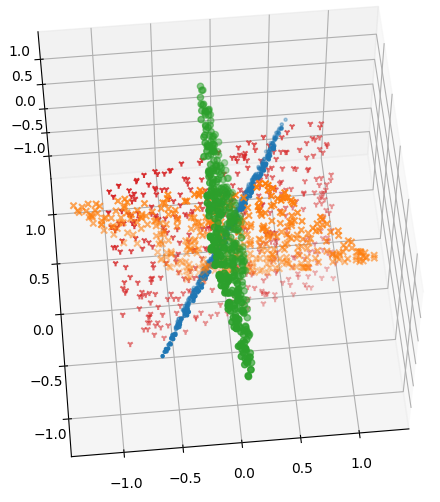
\includegraphics[width=\textwidth]{pics/points-400-400-400-400.png}
        \caption{Point cloud consisting of four planes with 400 points each and noise $\epsilon=0.01$.}
    \end{subfigure}%
    \hspace{2em}
    \begin{subfigure}{.45\textwidth}
        \centering
        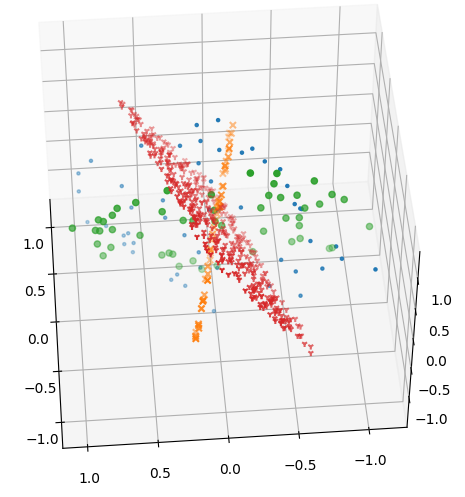
\includegraphics[width=\textwidth]{pics/points-50-50-50-400.png}
        \caption{Point cloud consisting of four planes, of which three have 50 points and one has 400 points with noise $\epsilon=0.01$.}
    \end{subfigure}
    \caption{Two possible point clouds.} \label{fig:point_cloud_examples}
\end{figure}


\bibliography{main}{}
\bibliographystyle{plain}

\end{document}